\documentclass[a4paper,twoside,11pt]{report}
\usepackage[italian]{babel}
\usepackage[utf8x]{inputenc}
%\usepackage[latin1]{inputenc}
\usepackage[T1]{fontenc}
%\usepackage[scaled]{helvet}
%\renewcommand\familydefault{\sfdefault}

%\renewcommand{\sfdefault}{cmr}
%helvetica
%\renewcommand{\sfdefault}{phv}
%courier
%\renewcommand{\sfdefault}{pcr}

\usepackage{caption}
\usepackage{subcaption}
\usepackage{sidecap}

\usepackage{quoting}
\quotingsetup{font=small}

\usepackage{eurosym}
\usepackage{graphicx}
\usepackage{epsfig}
\usepackage{url}
\usepackage{listings}
\usepackage{comment}
\usepackage{color}
\usepackage{amsmath}
\usepackage[dvipsnames]{xcolor}
%%https://en.wikibooks.org/wiki/LaTeX/Colors
\usepackage[colorlinks]{hyperref}
%\hypersetup{hidelinks}

%\lstset{
%	basicstyle=\ttfamily,
%	columns=fullflexible,
%	showstringspaces=false,
%	commentstyle=\color{gray}\upshape,
%	xleftmargin=\parindent,
%	belowcaptionskip=100\baselineskip,
%	basicstyle=\footnotesize\ttfamily	
%}

%\definecolor{forestGreen}{RGB}{34,139,34}
%\definecolor{backcolour}{rgb}{0.95,0.95,0.92}
%\definecolor{dkgreen}{rgb}{0,0.6,0}
%\definecolor{gray}{rgb}{0.5,0.5,0.5}
%\definecolor{mauve}{rgb}{0.58,0,0.82}

\definecolor{lightgray}{rgb}{0.95,0.95,0.90}
\definecolor{darkgray}{rgb}{.4,.4,.4}
\definecolor{azure}{rgb}{0.0, 0.5, 1.0}

\hypersetup{%
	,urlcolor=azure
	,citecolor=lightgray
	,linkcolor=darkgray
}

%\lstdefinelanguage{XML}
%{
%	basicstyle=\scriptsize,
%	sensitive=true,
%	showstringspaces=false,
%	numbers=left,
%	numberstyle=\tiny,
%	tabsize=4,
%	numbersep=3pt,
%	extendedchars=true,
%	xleftmargin=2em,
%	lineskip=1pt,
%	breaklines,
%	captionpos=t,
%	backgroundcolor=\color{lightgray},
%	morekeywords={android},
%	alsoletter={:,,/,?},
%	morestring=[b]{"},
%	morecomment=[s]{&lt;!--}{--&gt;},
%	keywordstyle=\color{forestGreen},
%	identifierstyle=\color{blue}\ttfamily,
%	stringstyle=\color{orangeRed}\ttfamily,
%	commentstyle=\color{forestGreen}\ttfamily
%}

%\lstset
%{ 	
%	language=Bash,
%	basicstyle=\scriptsize,
%	sensitive=true,
%	showstringspaces=false,
%	numbers=none,
%	numberstyle=\tiny,
%	tabsize=4,
%	numbersep=3pt,
%	extendedchars=true,
%	xleftmargin=2em,
%	lineskip=1pt,
%	breaklines,
%	captionpos=t,
%	backgroundcolor=\color{lightgray},
%	morestring=[b]{"},
%	morecomment=[l]{\#},
%	keywordstyle=\color{forestGreen},
%%	identifierstyle=\color{codegreen}\ttfamily,
%	stringstyle=\color{codepurple}\ttfamily,
%	commentstyle=\color{codegray}\ttfamily
%}

\definecolor{codeorange}{rgb}{1,0.5,0}
\definecolor{codegreen}{rgb}{0,0.6,0}
\definecolor{codegray}{rgb}{0.5,0.5,0.5}
\definecolor{codepurple}{rgb}{0.58,0,0.82}
\lstset{
	language=Java,
	basicstyle=\footnotesize\ttfamily,
	breaklines=true,
	breakatwhitespace=true,
	xleftmargin=\parindent,
	showstringspaces=false,
	sensitive=true,
	lineskip=1pt,
	numberstyle=\tiny,
	belowcaptionskip=1\baselineskip,
	tabsize=4,
	numbersep=3pt,
	extendedchars=true,
	keywordstyle=\bfseries\color{codeorange},
	commentstyle=\itshape\color{codepurple},
	identifierstyle=\color{codegray},
	stringstyle=\bfseries\color{codegreen},
	backgroundcolor=\color{lightgray}
}


%belowcaptionskip=100\baselineskip,
%xleftmargin=\parindent, 

%\lstset{
%	basicstyle=\ttfamily,
%	columns=fullflexible,
%	showstringspaces=false,
%	commentstyle=\color{codegreen}\upshape
%}

%opening
\title{Ingegneria dei Sistemi Software
	\\ Adattativi Complessi
	\\{\Large Stima della distanza utilizzando tecnologie BLE}}
\author{Federico Torsello - Matr. 702619}

\begin{document}
	\maketitle
	\tableofcontents
	%\listoffigures
	%\listoftables
	%\lstlistoflistings
	\begin{abstract}

\begin{description}
	\item [Capitolo 1] In questo capitolo si viene introdotti al progetto, quindi vengono descritti la vision e i goals.
	
	\item [Capitolo 2] In questo capitolo si definiscono ed analizzano i requisiti funzionali e non funzionali, i casi d'uso e i scenari relativi al progetto.
	
	\item [Capitolo 3] In questo capitolo si analizza brevemente la tecnologia iBeacon ed in generale il BLE (Bluetooth Low Energy). Sono inoltre forniti alcuni esempi di utilizzo reali e caratteristiche del protocollo di comunicazione.
	
	\item [Capitolo 4] In questo capitolo si definisce cos'è RSSI, come calcolarlo e come sfruttarlo per stimare la distanza utente-iBeacon target.
	
	\item [Capitolo 5] In questo capitolo si affronta la stima della distanza con RSSI, Android e tecnlogie Bluetooth Low Energy. In particolare si introduce all'utilizzo della libreria AltBeacon e di filtri su RSSI e sulle distanze stimate.
	
	\item [Capitolo 6] In questo capitolo si parla della stima della distanza utilizzando Arduino, prima con un progetto di test con questo connesso al PC e poi con l'implementazione legata all'app. Nel dettaglio si parlerà di come è possibile connettere direttamente l'Arduino allo smartphone per ricevere dati sensoristici.
	
	\item [Capitolo 7] In questo capitolo si struttura il progetto facendo l'analisi delle classi più alcuni codici sorgente di esempio.
	
	\item [Capitolo 8] In questo capitolo si passa all'implementazione vera e propria dell'app, riportando immagini e descrizioni per del suo utilizzo.
	
	\item [Capitolo 9] In questo capitolo si definisce il testing reale della stima delle distanze e gli strumenti necessari per eseguirlo.
\end{description}

\end{abstract}
	\chapter{Introduzione}

	Stimare con precisione la distanza che intercorre tra un utente ed un punto target è, secondo molti, una sfida tecnologica. Sempre più sistemi	 con applicazioni mobile e non necessitano di questa informazione per poter funzionare in modo corretto. 
	
	Per stimare la distanza esistono diverse tecnologie più o meno precise e costose. In questo senso l'avvento delle tecnologie IoT (\textit{Internet of things}) ha influito positivamente abbassando il costo dell'hardware necessario, creando community di hobbisti e professionisti, quindi ampliando il numero di librerie software (spesso open source) disponibili e progetti da cui prendere spunto.
	
\section{Vision}

\begin{itemize}
	\item Realizzare un sistema software mobile per stimare al meglio la distanza che intercorre tra l'utente e gli iBeacon disposti in un ambiante indoor.
	
	\item Utilizzare solo tecnologie open source per realizzare il tutto, ribadendone l'utilità e l'efficienza.
\end{itemize}

\section{Goals}
\subsection{\underline{Goals principali}}
\begin{enumerate}
	\item Sviluppare un'app Android in grado di interagire con degli iBeacon disposti in una stanza.
	
	\item Realizzare un'app compatibile con tutte le API Android 18 e superiori.
	
	\item L'app deve utilizzare i valori RSSI dei iBeacon per determinare la distanza trasmettitore-ricevitore.
	
	\item Implementare diversi filtri per ridurre gli effetti indesiderati del \textit{multipath fading} sulla stima della distanza.
	
	\item Realizzare e testare un \textbf{filtro di Kalman}, un \textbf{filtro ARMA} (\textit{Auto Regressive Moving Average}) e un \textbf{filtro RunningAverageRssi} per limitare gli effetti indesiderati sopracitati.
	
	\item Visualizzare dei grafici sull'app che in tempo reale descrivano l'andamento della distanza stimata.
	
	\item Curare la \textit{User Experience} realizzando una GUI chiara e responsive utilizzando librerie \textit{com.android.support}
	
	\item Sviluppare l'intero sistema utilizzando GNU/Linux e FOSS (Free and open-source software).
\end{enumerate}

\subsection{\underline{Goals secondari}}
\begin{enumerate}	
	\item Realizzare un programma C++/Wiring in grado di determinare la distanza percepita da un sensore ultrasonico collegato ad una board Arduino.
	
	\item Realizzare un mini progetto per testare il sensore ultrasonico. Nello specifico si considera un Arduino connesso al PC attraverso la porta USB e una view di feedback per visualizzare a schermo la distanza "reale".
	
	\item Abilitare la comunicazione seriale mediante tecnologia \textbf{USB OTG}, facendo diventare lo smartphone un host USB.
	
	\item Implementare la visualizzazione della distanza percepita dall'Arduino direttamente nell'app. L'obiettivo è dare un feedback della reale distanza iBeacon-utente e poterla mettere a confronto con quella stimata utilizzando gli RSSI. 
	
	In questo caso si considera un \textbf{Arduino connesso allo smartphone} attraverso la porta USB.
\end{enumerate}




	\chapter{Requisiti}

\section{Requisiti funzionali}
Per la realizzare del sistema si necessita:
\begin{itemize}
	\item di un utente in possesso di uno smartphone con sistema operativo Android versione 4.3 o superiore;
	
	\item uno o più iBeacon;
	
	\item un ambiente chiuso (come una stanza) in cui disporre gli iBeacon.
\end{itemize}
Nello specifico, per non alterare la ricezione dei segnali inviati dagli iBeacon, questi devono essere disposti:
\begin{itemize}
	\item su pareti regolari a circa 1 metro da terra;
	
	\item lontano da apparecchi che emettono onde elettromagnetiche (ad esempio router wifi);
	
	\item al sicuro da raffiche di vento;
	
	\item in aree in cui non si frappongano oggetti o persone tra lo smartphone e l'iBeacon target.
\end{itemize}

\section{Requisiti funzionali secondari}
Per poter avere un feedback a schermo della distanza reale utente-iBeacon si necessita di:
\begin{itemize}
	\item una board Arduino UNO (o superiore);
	
	\item un sensore ultrasonico;
	
	\item cavi di collegamento maschio-femmina;
	
	\item un cavo USB da stampante;
	
	\item uno smartphone che supporti la tecnologia \href{https://it.wikipedia.org/wiki/USB_On-The-Go}{\textbf{USB OTG (\textit{On-The-Go})}}\footnote{USB OTG - \url{https://it.wikipedia.org/wiki/USB_On-The-Go}}
	
	\item un cavo USB OTG.
\end{itemize}

%\section{Requisiti non funzionali}
%???

\section{Analisi dei requisiti}
\subsection{Casi d'uso}
\begin{figure}[ph]
	\centering
	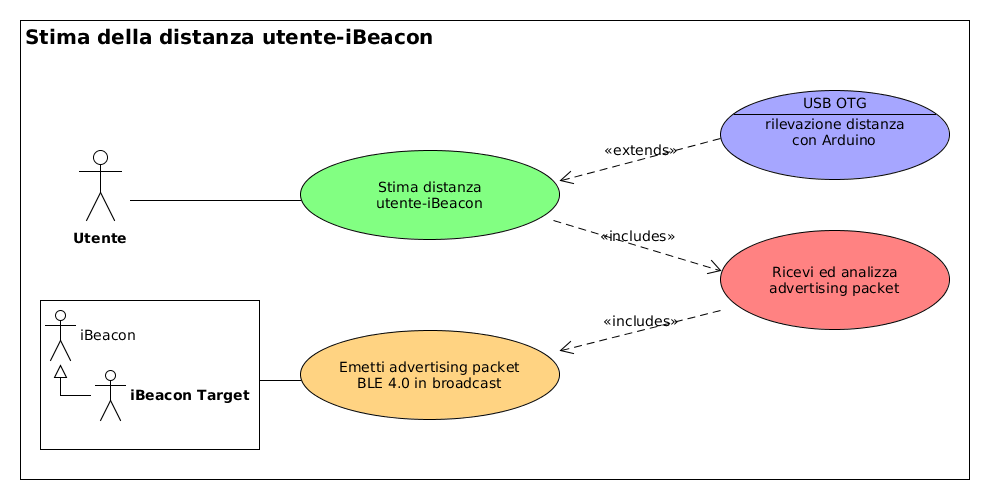
\includegraphics[scale=.45]{img/uml/use_case/use_case1}
	\caption[Use case - Stima della distanza utente-iBeacon]{Use case - Stima della distanza utente-iBeacon}
	\label{fig:usecase}
\end{figure}

\subsection{Scenari}

\subsubsection{\underline{Scenario classico}}
Nello scenario classico l'utente utilizza l'app per scansionare l'ambiente alla ricerca di iBeacon e leggere delle informazioni a schermo.

Nello specifico in questo scenario:
\begin{itemize}
	\item Si considera un utente in una stanza con uno smartphone Android in mano.
	
	\item La stanza in questione può presentare uno o più iBeacon disposti sui muri ad un'altezza di circa 1 metro dal suolo.
	
	\item Sullo smartphone viene avviata l'app.
	
	\item Nel caso in cui la radio Bluetooth dello smarphone fosse spenta o si dovesse spegnere, l'app stessa la accenderà/riaccenderà indicando all'utente l'avvenuto switch.
	
	\item L'utente preme su un bottone per avviare la scansione degli iBeacon presenti.
	
	\item Se vengono rilevati iBeacon corrispondenti con la lista di indirizzi MAC presente nell'app, allora viene caricata una lista di informazioni a schermo (\textit{friendly name}, immagine, distanza stimata, ecc\dots).
\end{itemize}

\subsubsection{\underline{Scenario classico avanzato}}
\begin{itemize}
	\item Una volta che l'utente ha visualizzato l'iBeacon di suo interesse (detto \textit{target}), lo seleziona dalla lista facendo click sull'item corrispondente.
	
	\item A questo punto all'utente vengono proposti solo i dettagli relativi al target, isolandoli dagli altri.
	
	\item In questa sezione l'utente potrebbe visualizzare un feedback della distanza reale (se tutte le condizioni a contorno sono soddisfatte) in metri.
	
	\item Trascinando il dito da destra a sinistra all'utente viene proposta un'altra area ancora più dettagliata dove è possibile mettere a confronto le varie stime della distanza (filtrata, non filtrata e reale se presente), in dei grafici realizzati in tempo reale.
\end{itemize}

	\chapter{Stima della distanza con RSSI}

\section{Attenuazione dei segnali elettromagnetici}
Il fenomeno dell'\textbf{attenuazione} dei segnali elettromagnetici si manifesta nella decrescita della potenza di segnale ricevuto dal ricevitore in relazione all’aumentare della distanza dalla sorgente emittente di tale segnale.

Nota questa relazione, se si conosce la potenza di segnale del trasmettitore \textbf{P} è possibile creare un modello per legare l'\textbf{\textit{attenuazione di segnale}} \textbf{A} e la distanza col ricevitore al fine di stimare la \textbf{\textit{distanza relativa}} trasmettitore-ricevitore \textbf{d}.
\begin{equation}\label{eq:realazione_potenza_segnale}
	P = f(d) 
\end{equation}

\section{Received Signal Strength Indicator - RSSI}
Per stimare la distanza relativa tra trasmettitore e ricevitore si può sfruttare l'attenuazione di segnale indicata dal valore RSSI il cui calcolo è poco costoso e non necessita di hardware aggiuntivo. 

RSSI è utile per smartphone che implementano radio Bluetooth in quanto permette di sviluppare proximity app o localizzazione indoor. Il suo valore viene calcolato in automatico dal sistema operativo dello smartphone.

Purtroppo questo approccio non è particolarmente preciso in quanto l’ambiente influisce sulla potenza del segnale ricevuto e quindi sull'attenuazione reale che rende il valore RSSI oscillante.

\begin{figure}[!ht]
	\centering
	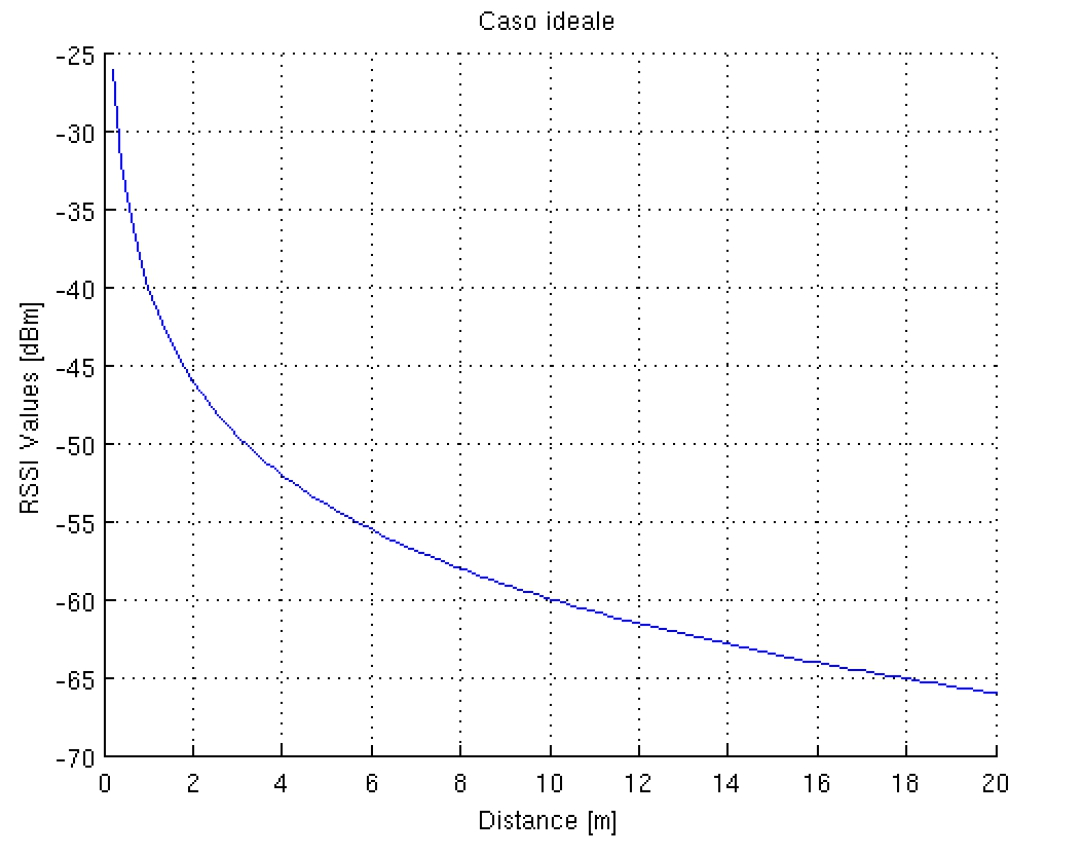
\includegraphics[scale=.25]{img/algoritmi/RSS.png}
	\caption{RSSI - Modello dell'andamento di RSSI in funzione della distanza}
\end{figure}



\section{Calcolo di RSSI}
Per il calcolo di RSSI (in dBm) si assume:
\begin{enumerate}
	\item che un segnale radio emesso in nello spazio libero da ostacoli e rumore decade di un fattore $ d^{-2} $, dove \textbf{d} è la distanza relativa trasmettitore-ricevitore
	
	\item che la potenza media ricevuta attraverso un canale reale decade proporzionalmente a $ n = d^{-n} $ , dove \textbf{n} è detto \textbf{l’esponente path-loss}. Tipicamente \textit{n} è compreso tra 2 e 4.
\end{enumerate}

\subsection{Equazione di trasmissione di Friis}

La distanza dal trasmettitore viene valutata utilizzando l’\textbf{equazione di trasmissione di Friis}:

\begin{equation}\label{eq:potenza_ricevuta}
P_R = P_T \frac{G_T G_R  \lambda^2}{(4 \pi)^2 \textbf{d}^n}
\end{equation}
dove:

\begin{itemize}
	\item $ P_R $ : potenza del segnale ricevuto (espressa in Watt) 
	\item $ P_T $ : potenza del segnale trasmesso (espressa in Watt) 
	\item $ G_R $ : guadagno dell’antenna ricevente
	\item $ G_T $ : guadagno dell’antenna trasmittente
	\item $\lambda = \frac{v}{f}$ : lunghezza d’onda
	\subitem $ v $ : velocità di propagazione
	\subitem $ f $ : frequenza dell'onda 
	\item $ d $ : distanza in metri
	\item $ n $ : constante di propagazione del segnale che dipende dall’ambiente
\end{itemize}
L'equazione \eqref{eq:potenza_ricevuta} calcola il rapporto tra la potenza ricevuta da un'antenna e la potenza trasmessa, in condizioni ideali.

\subsection{Conversione della potenza}
Conversione dalla potenza espressa in watt alla potenza espressa in dBm

\begin{equation}\label{eq:1dBm}
	1_{[dBm]} = 0.001258925_{[W]}
\end{equation}

\begin{equation}\label{eq:1W}
	1_{[W]} = 30_{[dBm]}
\end{equation}

\begin{equation}\label{eq:potenza_in_dBm}
	P_{[dBm]} = 10\log_{10} (10^{3}P_{[W]}/1_{[W]})
\end{equation}

\subsection{Potenza media a distanza di riferimento $ d_0 $}
\begin{equation}\label{eq:potenza_media_a_distanza_d}
	P(d)_{[dBm]} = P_{0\;[dBm]} \left(\frac{d}{d_0} \right)^{-n}
\end{equation}

dove $ P_0 $ è la potenza ricevuta (dBm) a una piccola distanza di riferimento $ d_0 $.

\subsection{Equazione di RSSI}
Combinando la \eqref{eq:potenza_ricevuta} e la \eqref{eq:potenza_in_dBm}, applicando le proprietà dei logaritmi si ottiene:
\begin{equation}
RSSI = −(10\,n\log_{10} \textbf{d} − A)
\end{equation}

dove \textit{A} è la potenza del segnale ricevuto (dBm) a distanza di un metro considerando una costante di propagazione \textit{n}.

\section{Calcolo della distanza}
La seguente equazione permette di stimare la distanza tra l'utente ed un target conoscendo il valore RSSI ed i parametri \textit{A} ed \textit{n}:

\begin{equation}\label{key}
RSSI = P - 10 * n * \log_10(d)
* n = 2 (in free space)
* d = 10 ^ ((TxPower - RSSI) / (10 * n))
\end{equation}

\begin{equation}
\textbf{d} = 10 \left( \frac{A − RSSI}{10\,n} \right)
\end{equation}

Con questa formula si può stimare la distanza .





\section{Problematiche della stima della distanza con RSSI}
I principali fenomeni negativi che inficiano l'utilizzo di RSSI come approccio per determinare la distanza tra due punti sono:
\begin{itemize}
	\item \textbf{Riflessione:} il segnale si propaga anche attraverso un percorso riflesso, provocando un \textbf{multi-path fading}. Al ricevitore giungono segnali con ampiezze e fasi differenti che vanno a sommarsi o sottrarsi in funzione della frequenza, causando un fading selettivo. Può essere causato da metalli e altri materiali riflettenti.
	\item \textbf{Intralcio:} shadowing che altera il normale decadimento dell’intensità che si avrebbe in spazio libero. L’attenuazione improvvisa del segnale è causata degli ostacoli (mobili, muri, alberi, edifici, ecc.) nel cammino trasmettitore-ricevitore
	\item \textbf{Assorbimento:} oggetti, come elementi liquidi o corpi umani, che assorbono la potenza del segnale.
	\item \textbf{Altezza:} la differenza di altezza può falsare la stima
	\item \textbf{Orientamento relativo:} il segnale decade se il ricevitore non è direzionato verso l'emettitore
\end{itemize}

\begin{figure}[!ht]
	\centering
	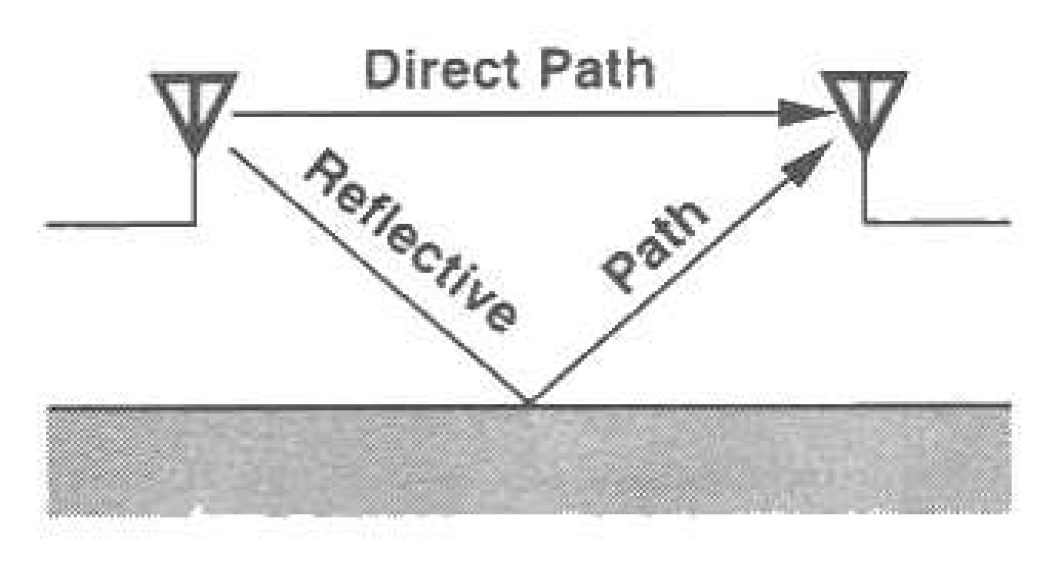
\includegraphics[scale=.16]{img/algoritmi/RSS_PROBLEMI.png}
	\caption{RSSI - Problemi di riflessione}
\end{figure}


 
 

	\chapter{Stima della distanza con Arduino}
\section{Progetto per stimare la distanza con un sensore ultrasonico ed un Arduino}
Per poter stimare la distanza con Arduino è stato utilizzato un sensore ultrasonico. Questo sensore è stato connesso direttamente alla board attraverso cavi maschio-femmina.

Per 

\begin{itemize}
	 \item Implementare un progetto Arduino che faccia uso della libreria \href{http://playground.arduino.cc/Code/NewPing}{\textbf{NewPing}}\footnote{\href{http://playground.arduino.cc/Code/NewPing}{\textbf{NewPing}} - \url{http://playground.arduino.cc/Code/NewPing}};
	 
	 \item Sfruttare la libreria \href{https://github.com/mik3y/usb-serial-for-android}{\textbf{usb-serial-for-android}}\footnote{\href{https://github.com/mik3y/usb-serial-for-android}{\textbf{usb-serial-for-android}} - \url{https://github.com/mik3y/usb-serial-for-android}} per connettere l'Arduino ad Android e ricevere i dati seriali in tempo reale.
	 
	 \item Sviluppare un mini progetto su \href{https://netbeans.org/}{\textbf{NetBeans}}\footnote{\href{https://netbeans.org/}{\textbf{NetBeans}} - \url{https://netbeans.org/}} ed impiegare la libreria \href{https://github.com/scream3r/java-simple-serial-connector}{\textbf{jSSC}}\footnote{\href{https://github.com/scream3r/java-simple-serial-connector}{\textbf{jSSC}} - \url{https://github.com/scream3r/java-simple-serial-connector}} (\textit{java-simple-serial-connector}) per testare il sensore di prossimità collegando l'Arduino al PC e visualizzando la distanza a schermo.
\end{itemize}

\subsubsection{\underline{\href{http://playground.arduino.cc/Code/NewPing}{NewPing}}}\label{sec:newping}
\textbf{Caratteristiche}
\begin{itemize}
	\item Compatibile con diversi modelli di sensori ad ultrasuoni: SR04, SRF05, SRF06, DYP-ME007 e Parallax Ping™.
	
	\item Non soffre di \textbf{lag} di un secondo se non si riceve un ping di eco.
	
	\item Produce un ping coerente e affidabile fino a 30 volte al secondo.
	
	\item Timer interrupt method per sketch event-driven.
	
	\item Metodo di filtro digitale built-in \texttt{ping\_median()} per facilitare la correzione degli errori.
	
	\item Utilizzo dei registri delle porte durante l'accesso ai pin per avere un'esecuzione più veloce e dimensioni del codice ridotte.
	
	\item Consente l'impostazione di una massima distanza di lettura del ping "in chiaro".
	
	\item Facilita l'utilizzo di più sensori.
	
	\item Calcolo distanza preciso, in centimetri, pollici e uS.
	
	\item Non fa uso di \texttt{pulseIn}, metodo che risulterebbe lento e che con alcuni modelli di sensore a ultrasuoni restituisce risultati errati.
	
	\item Attualmente in sviluppo, con caratteristiche che vengono aggiunte e bug/issues affrontati.
\end{itemize}

\section{Progetto di test della comunicazione seriale PC - Arduino}
Il metodo più importante di questo mini progetto è \texttt{updateDistance()}. Questo metodo è di tipo \textbf{void}. Il suo scopo è quello di riceve in input i \textit{byte} dalla porta seriale e convertirli in stringhe da visualizzare a schermo su una \textit{jLabel}.

Per poter fare I/O sulla porta seriale si deve istanziare e configurare l'oggetto SerialPort, abilitando la comunicazione via USB con una board Arduino.

Per avviare la comunicazione:
\begin{itemize}
	\item si settano i parametri di ingaggio (baund rate, numero di bit dei pacchetti, numero dei bit di stop e se è presente un controllo di parità)
	
	\item si imposta l'event mask in modo da controllare se sul canale sono prenti \textit{char}
	
	\item si registra l'istanza di SerialPort in un listener di eventi di I/O della seriale per poi considerare solo i dati di tipo \textit{char} e scartare tutti gli altri. 
\end{itemize}


Metodo updateDistance()
\begin{lstlisting}[language=Java]
private void updateDistance() {    
	SerialPort serialPort = new SerialPort("/dev/ttyACM0");
	try {
		serialPort.openPort();
		
		serialPort.setParams( 
			SerialPort.BAUDRATE_115200, 
			SerialPort.DATABITS_8, 
			SerialPort.STOPBITS_1,
			SerialPort.PARITY_NONE);
			
		serialPort.setEventsMask(SerialPort.MASK_RXCHAR);
		
		serialPort.addEventListener((SerialPortEvent serialPortEvent) -> {
			if (serialPortEvent.isRXCHAR()) {
				try {
					Thread.sleep(20);
					String distance = serialPort.readString();
					jLabel1.setText(distance);
				} catch (SerialPortException | InterruptedException ex) {
				}
			}
		});
	} catch (SerialPortException ex) {
		System.out.println("SerialPortException: " + ex.toString());
	}
}
\end{lstlisting}


	\begin{itemize}
		
	
	\item Interagire con gli iBeacon sfruttando la libreria \href{https://github.com/AltBeacon/android-beacon-library}{\textbf{AltBeacon}}\footnote{\href{https://github.com/AltBeacon/android-beacon-library}{\textbf{AltBeacon}} - \url{https://github.com/AltBeacon/android-beacon-library}}.
	
	\item Implementare un \textbf{filtro di Kalman} per ridurre gli effetti indesiderati del \textit{multipath fading} sulla stima della distanza.
	
	\item Implementare un \textbf{filtro ARMA} (\textit{Auto Regressive Moving Average}) per stimare al meglio il valore RSSI.
	
	\item Implementare un \textbf{filtro RunningAverageRssi} da confrontare con i precedenti.
	
	\item Visualizzare grafici in tempo reale utilizzando la libreria \href{https://github.com/PhilJay/MPAndroidChart}{\textbf{MPAndroidChart}}\footnote{\href{https://github.com/PhilJay/MPAndroidChart}{\textbf{MPAndroidChart}} - \url{https://github.com/PhilJay/MPAndroidChart}}

	
\end{itemize}


%This filter calculates its rssi on base of an auto regressive moving average (ARMA) It needs only the current value to do this; the general formula is n(t) = n(t-1) - c * (n(t-1) - n(t)) where c is a coefficient, that denotes the smoothness - the lower the value, the smoother the average Note: a smoother average needs longer to "settle down" Note: For signals, that change rather frequently (say, 1Hz or faster) and tend to vary more a recommended value would be 0,1 (that means the actual value is changed by 10\% of the difference between the actual measurement and the actual average) For signals at lower rates (10Hz) a value of 0.25 to 0.5 would be appropriate
	\chapter{UML}

\section{Gerarchia delle classi}

\subsection{ApplicationActivity}
\begin{figure}[ph]
	\centering
	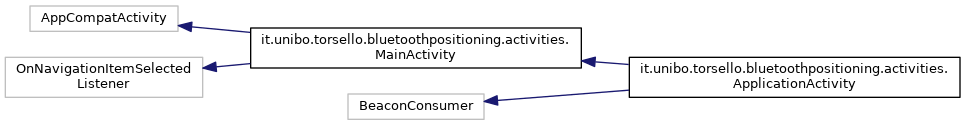
\includegraphics[width=1.1\linewidth]{img/uml/inherit_graph/inherit_graph_0.png}
	\caption[]{}
\end{figure}

\newpage

\subsection{Fragment e Observer}
\begin{figure}[ph]
	\centering
	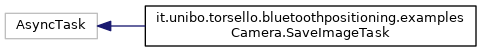
\includegraphics[scale=.55]{img/uml/inherit_graph/inherit_graph_10.png}
	\caption[]{}
\end{figure}

\subsection{Observable}
\begin{figure}[ph]
	\centering
	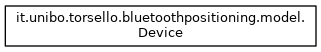
\includegraphics[scale=.55]{img/uml/inherit_graph/inherit_graph_14.png}
	\caption[]{}
\end{figure}

\newpage

\subsection{KFilter}
\begin{figure}[ph]
	\centering
	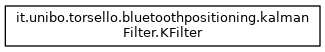
\includegraphics[scale=.55]{img/uml/inherit_graph/inherit_graph_11.png}
	\caption[]{}
\end{figure}

\subsection{KFilterBuilder}
\begin{figure}[ph]
	\centering
	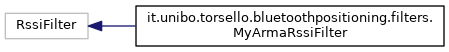
\includegraphics[scale=.55]{img/uml/inherit_graph/inherit_graph_12.png}
	\caption[]{}
\end{figure}

\subsection{MyArmaRssiFilter}
\begin{figure}[ph]
	\centering
	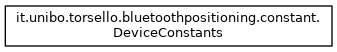
\includegraphics[scale=.55]{img/uml/inherit_graph/inherit_graph_4.png}
	\caption[]{}
\end{figure}

\newpage

\subsection{Estimation}
\begin{figure}[ph]
	\centering
	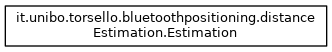
\includegraphics[scale=.55]{img/uml/inherit_graph/inherit_graph_8.png}
	\caption[]{}
\end{figure}

\subsection{Device}
\begin{figure}[ph]
	\centering
	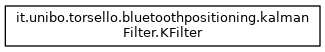
\includegraphics[scale=.55]{img/uml/inherit_graph/inherit_graph_13.png}
	\caption[]{}
\end{figure}

\subsection{DeviceCardViewAdapter}
\begin{figure}[ph]
	\centering
	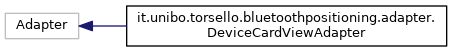
\includegraphics[scale=.55]{img/uml/inherit_graph/inherit_graph_1.png}
	\caption[]{}
\end{figure}

\newpage

\subsection{DeviceCardViewAdapter.DeviceViewHolder}
\begin{figure}[ph]
	\centering
	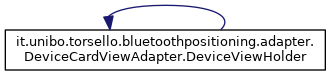
\includegraphics[scale=.55]{img/uml/inherit_graph/inherit_graph_2.png}
	\caption[]{}
\end{figure}

\subsection{StatePagerAdapter}
\begin{figure}[ph]
	\centering
	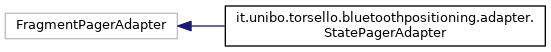
\includegraphics[scale=.55]{img/uml/inherit_graph/inherit_graph_3.png}
	\caption[]{}
\end{figure}

\newpage

\subsection{DeviceConstants}
\begin{figure}[ph]
	\centering
	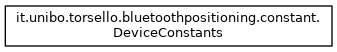
\includegraphics[scale=.55]{img/uml/inherit_graph/inherit_graph_5.png}
	\caption[]{}
\end{figure}

\subsection{KFilterConstants}
\begin{figure}[ph]
	\centering
	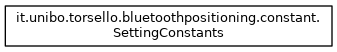
\includegraphics[scale=.55]{img/uml/inherit_graph/inherit_graph_6.png}
	\caption[]{}
\end{figure}

\subsection{SettingConstants}
\begin{figure}[ph]
	\centering
	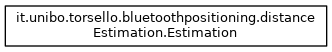
\includegraphics[scale=.55]{img/uml/inherit_graph/inherit_graph_7.png}
	\caption[]{}
\end{figure}

\newpage
\subsection{CameraPreviewUtil}
\begin{figure}[ph]
	\centering
	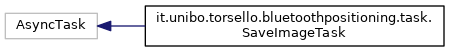
\includegraphics[scale=.55]{img/uml/inherit_graph/inherit_graph_16.png}
	\caption[]{}
\end{figure}

\subsection{SaveImageTask}
\begin{figure}[ph]
	\centering
	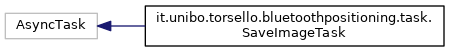
\includegraphics[scale=.55]{img/uml/inherit_graph/inherit_graph_15.png}
	\caption[]{}
\end{figure}

\subsection{ChartUtil}
\begin{figure}[ph]
	\centering
	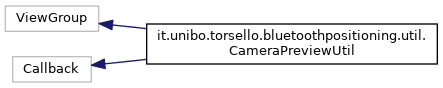
\includegraphics[scale=.55]{img/uml/inherit_graph/inherit_graph_17.png}
	\caption[]{}
\end{figure}

\newpage
\subsection{UsbUtil}
\begin{figure}[ph]
	\centering
	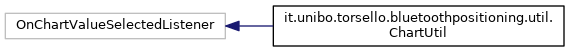
\includegraphics[scale=.55]{img/uml/inherit_graph/inherit_graph_18.png}
	\caption[]{}
\end{figure}

\subsection{FABBehavior}
\begin{figure}[ph]
	\centering
	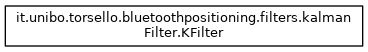
\includegraphics[scale=.55]{img/uml/inherit_graph/inherit_graph_9.png}
	\caption[]{}
\end{figure}

%	\include{analisi_del_problema}
%	\include{stima_distanza}
%	\include{work_plan}
%	\include{progetto}
	%\include{Grafi}
%	\begin{thebibliography}{9}
	\bibitem{}
	Matthew S. Gast,
	\textit{Building Applications with iBeacon}.
	
	\bibitem{}
	Stephen Statler,
	\textit{Beacon Technologies}.
	
	\bibitem{}
	Frode Eika Sndnes, Yan Zhang, Chunming Rong, Laurence T. Yang, Jianhua Ma,
	\textit{Ubiquitous Intelligence and Computing - 5th Internationa Conferende, UIC 2008, Spring}.
	
	\bibitem{}
	Ugur Bekcibasi,
	\textit{Increasing RSSI Localization Accuracy with Distance Reference Anchor in Wireless Sensor Networks}.

	
	\bibitem{}
	Luca Pappalardo, 
	\textit{Localizzazione - Problema, Tecniche, Algoritmi},
	\\Reti mobili: Ad Hoc e di sensori, 
	\\Slide, 2011.
	
	\bibitem{}
	Cuccado, De Franceschi, Fauri, Sartor,
	\textit{Analisi di algoritmi di autolocalizzazione per reti di sensori wireless},
	\\Tesi di laurea, 2011.
	
	\bibitem{}
	Paolo Sperandio,
	\textit{Algoritmi di localizzazione per reti di sensori wireless}
	\\Tesi di laurea, 2007.
	
	\bibitem{}
	Xuchen Yao,
	\textit{An Introduction to the Kalman Filter}.
	\\\url{http://www.cs.unc.edu/~welch/media/pdf/kalman_intro.pdf}
		
	\bibitem{}
	Ilenia Tinnirello,
	\textit{Un Esempio di Applicazione 	del Filtro di Kalman alle reti WiFi}.
	
	\bibitem{}
	Angelo Nunzio La Bruna,
	\textit{Applicazioni del filtro di Kalman su accelerometri}.
	
	\bibitem{}
	Philipp Jahoda,
	\textit{MPAndroidChart}
	\url{https://github.com/PhilJay/MPAndroidChart}
\end{thebibliography}
	
\end{document}